\documentclass{article}
\usepackage{cmap}
\usepackage[T2A]{fontenc}
\usepackage[utf8]{inputenc}
\usepackage[english, russian]{babel}
\usepackage[a4paper, left=10mm, right=10mm, top=12mm, bottom=15mm]{geometry}
\usepackage{mathtools,amssymb}
\usepackage{graphicx}

\linespread{1.4}

\newenvironment{task}{\begin{center}\fontsize{14}{14}\selectfont\bf}{\rm\fontsize{12}{12}\selectfont\end{center}}


\begin{document}
	\begin{center}
		Токмаков Александр, группа БПМИ165 \\
		Домашнее задание 4
	\end{center}
	
	\begin{task} 
		№1
	\end{task}
	Разбивая отрезок $[0, 1]$ на два отрезка, мы выбираем точку $x_0 \in [0, 1]$. При этом $M = max(x, 1-x)$, $m = min(x, 1-x)$. Пусть $\Omega = [0, 1]$ - вероятностное пространство, $P(x_0 \in A \subseteq [0,1]) = \int\limits \limits_{A} 1dx$ - вероятность того, что $x_0$ попадёт в некоторое множество $A$ (оно должно быть достаточно хорошим, чтобы интеграл посчитался, но это не важно). Очевидно, что длина меньшего отрезка всегда $< 0.5$, поэтому $P(m \leq a) = 1$ при $a \in (\frac{1}{2}, +\infty)$ и не может быть отрицательна, поэтому $P(m \leq a) = 0$ при $a \in (-\infty, 0)$. Зафиксируем некоторое $a \in [0, \frac{1}{2}]$. Отрезок длины $m \leq a$ получится если $x_0 \in [0, a]$ или если $x_0 \in [1-a, 1]$. Тогда
	$P(m \leq a) = \int\limits_0^a 1dx + \int\limits_{1-a}^1 1dx 
	= (a - 0) + (1 - (1-a)) = 2a$.



	\begin{task} 
		№8
	\end{task}
	Пусть вероятностное пространство - $\Omega = [0, 1]^2$ - множество точек квадрата со стороной 1, $P((x_0, y_0) \in A) = \iint\limits_{A}1dxdy$ - вероятность того, что равновероятно выбранная точка попала в некоторое подмножество $A$. \\
	
	\bf a) \rm Расстояние от точки до фиксированной стороны квадрата не превосходит $a$:\\
	Очевидно, что $P(\leq a) = 0$ при $a < 0$ и $P(\leq a)=1$ при $1<a$. При $0 \leq a \leq 1$: \\
	\begin{center}
	$A = \left\lbrace(x, y) \in \Omega \hspace{4px}|\hspace{4px} y \leq a \right\rbrace
       = \left\lbrace(x, y) \in \mathbb{R}^2 \hspace{4px}|\hspace{4px} 0\leq x \leq 1 \wedge 0 \leq y \leq a \right\rbrace$ \\
    $P(\leq a) = P(A) = \iint\limits_A1dxdy = \int\limits_0^1 \left( \int\limits_0^a 1dy \right)dx 
     = \int\limits_0^1 adx = a$

	\end{center}

	\bf a) \rm Расстояние от точки до ближайшей стороны квадрата не превосходит $a$:\\
	Очевидно, что $P(\leq a) = 0$ при $a < 0$ и $P(\leq a)=1$ при $\frac{1}{2}<a$. При $0 \leq a \leq \frac{1}{2}$: \\
	\begin{center}
		$A_1 = \left\lbrace(x, y) \in \Omega \hspace{4px}|\hspace{4px} x \leq a \wedge x \leq y \leq 1-x \right\rbrace
		= \left\lbrace(x, y) \in \mathbb{R}^2 \hspace{4px}|\hspace{4px} 0\leq x \leq a \wedge x \leq y \leq 1-x  \right\rbrace$ \\
		$P(A_1) = \iint\limits_{A_1}1dxdy = \int\limits_0^a \left( \int\limits_x^{1-x} 1dy \right)dx 
		= \int\limits_0^a (1 - 2x)dx = a - a^2$
	\end{center}
	Но это вероятность для одной стороны (случай, когда сторона $x = 0 \quad-$  ближайшая). Случаи, когда ближайшей окажется одни из трёх других сторон полностью аналогичны в силу симметрии, поэтому $P(\leq a) = 4\cdot P(A_1) = 4a - 4a^2$.

	\bf c) \rm Расстояние от точки до ближайшей диагонали квадрата не превосходит $a$:\\
	\begin{center} 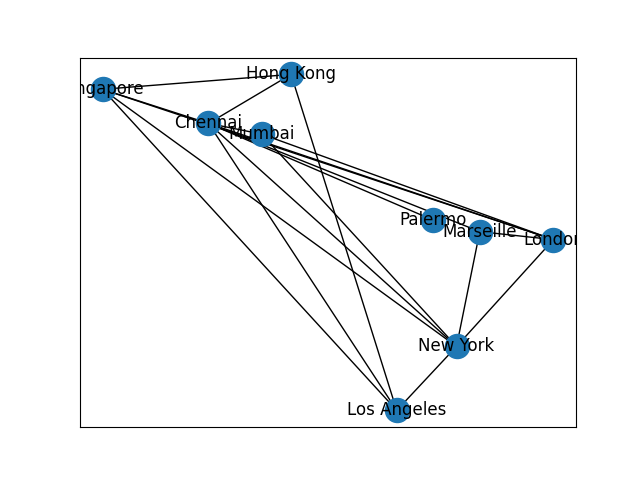
\includegraphics[width=11cm]{img} \end{center}
	Очевидно, что $P(\leq a) = 0$ при $a < 0$ и $P(\leq a)=1$ при $\frac{\sqrt{2}}{4}<a$. При $0 \leq a \leq \frac{\sqrt{2}}{4}$: \\
	\begin{center}
	$A1 = \left\lbrace(x, y) \in \Omega \hspace{4px}|\hspace{4px} x \leq \frac{1}{2} \hspace{4px}\wedge\hspace{4px} x - a\sqrt{2} \leq y \leq x \right\rbrace = A_{11} \cup A_{12}
	=$\\$= \left\lbrace(x, y) \in \mathbb{R}^2 \hspace{4px}|\hspace{4px} 0 \leq x < a\sqrt{2} \hspace{4px}\wedge\hspace{4px} 0 \leq y \leq x \right\rbrace 
	\cup \left\lbrace(x, y) \in \mathbb{R}^2 \hspace{4px}|\hspace{4px} a\sqrt{2} \leq x \leq \frac{1}{2} \hspace{4px}\wedge\hspace{4px} x - a\sqrt{2} \leq y \leq x \right\rbrace$ \\
	
	$P(A_1) = P(A_{11}) + P(A_{12}) =  \iint\limits_{A_{11}}1dxdy + \iint\limits_{A_{12}}1dxdy 
	= \int\limits_0^{a\sqrt{2}} \left( \int\limits_0^x 1dy \right)dx + \int\limits_{a\sqrt{2}}^{\frac{1}{2}} \left( \int\limits_{x-a\sqrt{2}}^x 1dy \right)dx = $\\
	$= \int\limits_0^{a\sqrt{2}} x dx + \int\limits_{a\sqrt{2}}^{\frac{1}{2}}  a\sqrt{2}dx 
	= a^2 + a\sqrt{2}\cdot(\frac{1}{2} - a\sqrt{2}) = a\frac{\sqrt{2}}{2} - a^2
	$
	
	\end{center}
	Всего 8 симметричных случаев, значит $P(<a) = P(A) = 8P(A_1) = a4\sqrt{2} - 8a^2$




	\begin{task} 
		№9
	\end{task}
	Пусть $\Omega = [0, 30]^2$ - вероятностное пространство, $P((x, y) \in A) = \iint\limits_A\frac{dxdy}{30\cdot30}$ - вероятность того, что пара время опоздания лектора $x$ и время опоздания студента $y$ окажется в некотором $A$.\\
	Студенту нужно либо не опоздать, либо опоздать на время не большее, чем лектор: 
	\begin{center}
		$A = A_1 \cup A_2 = \left\lbrace(x, y) \in \mathbb{R}^2 \hspace{4px}|\hspace{4px} 0 \leq x \leq 30 \wedge 0\leq y \leq 10 \right\rbrace \cup \left\lbrace(x, y) \in \mathbb{R}^2 \hspace{4px}|\hspace{4px} 10 < x \leq 30 \wedge 0 \leq y < x - 10 \right\rbrace$ \\
		$P(A) = P(A_1) + P(A_2) = \iint\limits_{A_1}\frac{dxdy}{30\cdot30} + \iint\limits_{A_2}\frac{dxdy}{30\cdot30} 
		= \int\limits\limits_0^{30} \left( \int\limits_0^{10} \frac{dy}{900} \right)dx + \int\limits_{10}^{30} \left( \int\limits_0^{x-10} \frac{dy}{900} \right)dx = $\\$ 
		= \int\limits_0^{30} \frac{1}{90}\cdot dx + \int\limits_{10}^{30}  \frac{x-10}{900}dx
		= \frac{3}{9} + \frac{1}{900}\left(\frac{30^2}{2} - \frac{10^2}{2} - 10\cdot30 + 10\cdot 10 \right) = \frac{5}{9}$
		
	\end{center}



	\begin{task} 
		№10
	\end{task}
	Пусть вероятностное пространство - $\Omega = \left\lbrace(x, y) \in \mathbb{R}^2 \hspace{4px}|\hspace{4px} x^2 + y^2 \leq 1 \right\rbrace$ - множество точек круга радиуса 1,\\ $P((x_0, y_0) \in A) = \iint\limits_{A}\frac{dxdy}{\pi}$ - вероятность того, что равновероятно выбранная точка попала в некоторое подмножество $A$. \\
	
	Очевидно, что $P(x\leq a) = 0$ при $a < -1$ и $P(x\leq a)=1$ при $1<a$. При $-1 \leq a \leq 1$: \\
	\begin{center}
		$A = \left\lbrace(x, y) \in \mathbb{R}^2 \hspace{4px}|\hspace{4px} x^2 + y^2 \leq 1 \wedge x \leq a \right\rbrace
		= \left\lbrace(x, y) \in \mathbb{R}^2 \hspace{4px}|\hspace{4px} -1 \leq x \leq a \hspace{4px}\wedge\hspace{4px} -\sqrt{1-x^2} \leq y \leq \sqrt{1-x^2} \right\rbrace$ \\
		
		$P(x\leq a) = P(A) = \iint\limits_{A}\frac{dxdy}{\pi} 
		= \int\limits\limits_{-1}^a \left( \int\limits\limits_{-\sqrt{1-x^2}}^{\sqrt{1-x^2}} \frac{dy}{\pi} \right)dx 
		= \frac{2}{\pi}\int\limits\limits_{-1}^a \sqrt{(1-x^2)} dx 
		= \frac{1}{\pi}\left( x\sqrt{1-x^2} + \arcsin x \right) \Biggr|_{-1}^a
		=$\\$= \frac{1}{\pi}\left( a\sqrt{1-a^2} + \arcsin a \right) - \frac{1}{\pi}\left( \arcsin(-1) \right)
		= \frac{1}{\pi}\left( a\sqrt{1-a^2} + \arcsin a \right) - \frac{1}{\pi}\left( - \frac{\pi}{2} \right)
		= \frac{1}{\pi}\left( a\sqrt{1-a^2} + \arcsin a \right) + \frac{1}{2}$\\
	\end{center}
	\begin{center}
		$P(x\leq a) = \frac{1}{\pi}\left( a\sqrt{1-a^2} + \arcsin a \right) + \frac{1}{2}$
	\end{center}
	В силу симметрии:
	\begin{center}
		$P(y\leq a) = \frac{1}{\pi}\left( a\sqrt{1-a^2} + \arcsin a \right) + \frac{1}{2}$
	\end{center}
	При $a = 0$ события независимы: 
	\begin{center}
		$P(x\leq 0) = P(y\leq 0) = \frac{1}{2}\quad $\\
		$P(x \leq 0 \wedge y \leq 0)  = \frac{1}{4} = P(x\leq 0)\cdot P(y\leq0)$
	\end{center}
	При $a = 1$ события независимы: 
	\begin{center}
		$P(x\leq 1) = P(y\leq 1) = 1\quad $\\
		$P(x \leq 1 \wedge y \leq 1)  = 1 = P(x\leq 1)\cdot P(y\leq1)$
	\end{center}
	При $a = -0.5$ события зависимы: 
	\begin{center}
		$P(x\leq -0.5) = P(y\leq -0.5) = \frac{1}{3} - \frac{\sqrt{3}}{4\pi}\quad $\\
		
		$P(x \leq -0.5 \wedge y \leq -0.5)  = \int\limits_{-\frac{\sqrt{3}}{2}}^{-\frac{1}{2}} \left( \int\limits\limits_{-\sqrt{1-x^2}}^{\sqrt{1-x^2}} \frac{dy}{\pi} \right)dx
		= \frac{2}{\pi}\int\limits_{-\frac{\sqrt{3}}{2}}^{-\frac{1}{2}} \sqrt{(1-x^2)}dx
		= \frac{1}{\pi}\left( x\sqrt{1-x^2} + \arcsin x \right) \Biggr|_{-\frac{\sqrt{3}}{2}}^{-\frac{1}{2}} = - \frac{\sqrt{3}}{8} - \frac{\pi}{12}\frac{\sqrt{3}}{8} + \frac{\pi}{6}$ \\
		$P(x \leq -0.5 \wedge y \leq -0.5)  =  \frac{\pi}{12}$\\
		
		$P(x \leq -0.5 \wedge y \leq -0.5) \not = P(x\leq -0.5) \cdot P(y\leq -0.5)$
	\end{center}
	
	
\end{document}
